\iffalse
\documentclass[journal,12pt,twocolumn]{article}
\usepackage{graphicx}
\usepackage[none]{hyphenat}
\usepackage[margin=0.5in]{geometry}
\usepackage[cmex10]{amsmath}
\usepackage{array}
\usepackage{booktabs}
\usepackage{gensymb}
\usepackage{textcomp}
\title{\textbf{Circle Assignment}}
\author{Manideep Parusha - FWC22004}
\date{\today}

\providecommand{\norm}[1]{\left\lVert#1\right\rVert}
\providecommand{\abs}[1]{\left\vert#1\right\vert}
\let\vec\mathbf
\newcommand{\myvec}[1]{\ensuremath{\begin{pmatrix}#1\end{pmatrix}}}
\newcommand{\mydet}[1]{\ensuremath{\begin{vmatrix}#1\end{vmatrix}}}
\providecommand{\brak}[1]{\ensuremath{\left(#1\right)}}

\begin{document}

\maketitle
\section*{Problem}
\paragraph{
\fi
	Show that the tangents of circle drawn at the ends of diameter are parallel.
	\begin{figure}[!ht]
		\centering
 \includegraphics[width=\columnwidth]{chapters/10/10/2/4/figs/plot_cir.png}
		\caption{}
		\label{fig:10/10/2/4}
  	\end{figure}
	\\
	\solution See Fig. 
		\ref{fig:10/10/2/4}.
	\iffalse
\section*{Solution}

\begin{figure}[h]
\centering
\includegraphics[width=\columnwidth]{figs/plot_cir.png}
\caption{Circle with tangents at ends of it's diameter}
\label{fig:cir_py}
\end{figure}

\subsection*{Construction}
Input taken for the construction of the Circle and the tangents is 'r' radius of the circle.

\begin{table}[h]
	\centering
\setlength\extrarowheight{2pt}
	\begin{tabular}{|c|c|c|}
		\hline
		\textbf{Symbol} & \textbf{Value} & \textbf{Description} \\
		\hline
		r & 10 & circle radius\\
		\hline
		O & $-\vec{u}$ & Center\\
		\hline
		A & \myvec{a_1\\a_2} & point A\\
		\hline
		B & \myvec{b_1\\b_2} & point B\\
		\hline
	\end{tabular}
\end{table}

Let us assume a circle with radius 'r' and center at origin.\\
\begin{align}
	\vec{x}^{T}\vec{Vx} + 2\vec{u}^{T}\vec{x} + f = 0
\end{align}
but, for a Circle 
\begin{align}
	\vec{V} = \myvec{ 1 & 0 \\0 & 1}
\end{align}
and the center of the circle is,
\begin{align}
	-\vec{u} = \myvec{u_1 \\ u_2}
	\label{center}
\end{align}
\fi
Let $\vec{A}, \vec{B}$ be  the end points of the diameter of the circle through which the tangents are drawn.
From 
	\eqref{eq:circ-cr},
\begin{align}
	\frac{\vec{A} + \vec{B}}{2} = -\vec{u} \\
	\implies \vec{A}+\vec{B} = -2\vec{u}
	\label{ab}
\end{align}

From 
  \eqref{eq:conic_tangent_mq},
  \begin{align}
	  \vec{m}_1^{\top}\brak{\vec{A}+\vec{u}} &= 0
	  \\
	  \vec{m}_2^{\top}\brak{\vec{B}+\vec{u}} &= 0
  \end{align}
where $\vec{m_1}, \vec{m_2}$ are the direction vectors of the tangents at $\vec{A}, \vec{B}$ respectively.
Then, the normal vectors at the point of contact of tangets are
\begin{align}
	\vec{A}+\vec{u} &= k_1\vec{n_1}
	\label{n1}
	\\
	\vec{B}+\vec{u} &= k_2\vec{n_2}
	\label{n2}
\end{align}
Adding \eqref{n1} and \eqref{n2}, 
\begin{align}
	k_1\vec{n_1}+k_2\vec{n_2} &=\vec{A}+\vec{B} + 2\vec{u}  
	\\
	&=\vec{0}
	\label{addeq}
\end{align}
from \eqref{ab}, \eqref{addeq} can be expressed as 
 \begin{align}
	 k_1\vec{n_1}+k_2\vec{n_2} &= 0 \\
	 k_1\vec{n_1} &= -k_2\vec{n_2}
 \end{align}
Since 
\begin{align}
	\vec{n_1} \times \vec{n_2} &= \vec{0},
	\\
	\vec{n_1} \parallel \vec{n_2}  &\implies 
	\vec{m_1} \parallel \vec{m_2}  
\end{align}
\iffalse

 So the tangents are parallel to each other.\\
Hence, we have proved that the tangents at the ends of the diameter of a circle are parallel.
\end{document}
\fi
